In this chapter, we describe the details about the implementation of our approach to create the dynamic benchmark. The source code of this implementation is present on GitHub at \url{https://github.com/sola-st/master-thesis-piyush-bajaj/tree/automation}
We use various tools and libraries to make the benchmark accomplish the goals of being ready-to-run, ready-to-analyze, versatile, extensible and diverse and large-scale.
We describe these tools and libraries in the following sections.

\section{Source for Corpus of Projects}
\label{impl:corpus of projects}
As mentioned in the approach, we select the projects belonging to the different application domains from a predefined set of 679 projects from the the awesome python project.
In this work, we use the table of contents as shown in the Figure \ref{fig:awesome-python-website} to be the application domain for our selection process.
The figure \ref{fig:awesome-python-website} also shows the projects listed under the categories of Email, Enterprise Application Integration and Environment Management.
The category of Email further breaks down the projects into 3 sub-categories of Mail Servers, Clients and Others.
The GitHub repository of awesome python as well as the accompanying website can be accessed at \url{https://github.com/vinta/awesome-python/}.
We get source code of the project from GitHub repository which is provided by awesome python or the project website.  

\begin{figure}
    \centering
    \includegraphics[width=1\linewidth, height=1\linewidth]{figures/implementation/Awesome-Python-website3.png}
    \caption{Awesome Python Website}
    \label{fig:awesome-python-website}
\end{figure}

\section{First 5 Projects}
\label{impl:first five}
We start by manually selecting a random project from one of the categories in the awesome python corpus.
Then the number of stars for the repository on GitHub is checked. 
If the project has less than 500 stars we choose another random project, otherwise we proceed with the selected project.
This helps us to ensure the GitHub stars selection criteria mentioned in section \ref{approach:selection criteria}.
We proceed by cloning the source code of the project and installing it in a python virtual environment.
If the project is successfully installed, we add the pytest library to the virtual environment.
Finally, the test suite of the project is run using pytest. 
The project is chosen only if the execution is successful ensuring the selection criteria of presence and execution of test suite is met.

All of the above mentioned steps, from selecting a random project to running the test suite is performed a number of times to collect 5 different projects. 
Each time a random project is selected, we ensure that it does not belong to any of the categories that have been chosen before.
This helps us fulfill the selection criteria of diverse domain mentioned in section \ref{approach:selection criteria}.
Some library and dependency requirements were fixed during installation and execution of the projects.
Table \ref{table:first_5_projects} shows a list the projects which were chosen for installation till 5 of them satisfied all the selection criteria.

\begin{table}[ht]
    \centering
    \begin{tabular}{lllll}
    \hline
    \textbf{Category} & \textbf{Sub-category} & \textbf{Name} & \textbf{GitHub Stars} & \textbf{Criteria}\\
    \hline
    Web Crawling & - & grab & 2.2k & Yes\\
    DevOps Tools & SSH-style Deployment & fabric & 13.7k & No\\
    Robotics & - & PythonRobotics & 16.8k & Yes\\
    RESTful API & Flask & flask-api & 1.3k & Yes\\
    Deep Learning & - & mxnet & 20.2k & No\\
    Machine Learning & - & gym & 29k & No\\
    Job Scheduler & - & schedule & 10.2k & Yes\\
    Image processing & - & pagan & 278 & No\\
    Image Processing & - & pillow & 10.3k & Yes\\
    \hline
    \end{tabular}
    \caption{First 5 Projects for DyPyBench (Criteria : Test Suite Execution)}
    \label{table:first_5_projects}
\end{table}

\section{Automation for Installation}
\label{impl:automation}
Manual installation of projects as described in section \ref{impl:first five} shows us that the tasks of installation and execution are repetitive for each project with some exceptions.
These tasks become tedious and error prone, when we need to repeat them for 50 projects.
We automate these tasks using bash scripts which support loops for repetition and exceptions using conditionals.
The Figure \ref{fig:setup difference} shows the installation steps for two projects that satisfied the selection criteria.
The blue colored text indicate similarities, whereas the red colored text indicate the differences.

\begin{figure}[ht]
    \centering
    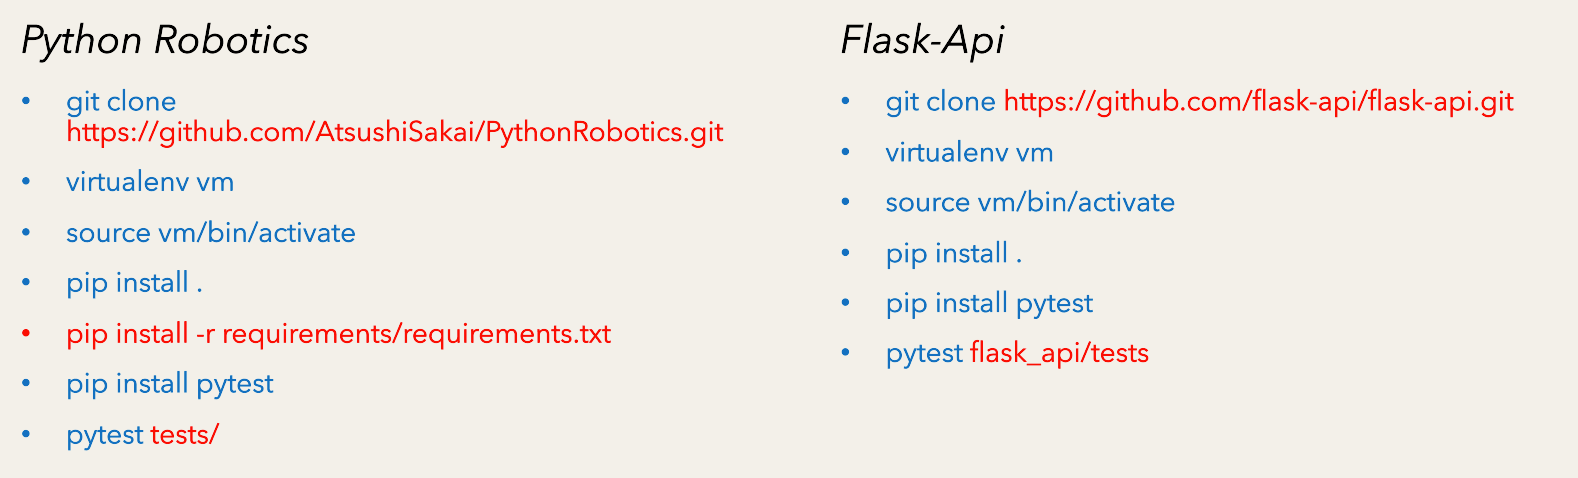
\includegraphics[width=1\linewidth]{figures/implementation/Setup-difference.png}
    \caption{Execution of Projects (Similarities and Differences)}
    \label{fig:setup difference}
\end{figure}

As can be seen from the Figure \ref{fig:setup difference}, the two commands of \textbf{git clone} and \textbf{pytest} have different argument values depending on the project.
To handle these difference we provide arguments to the bash script based on the project thereby making the automation generic.
These arguments are present in a text file, which is read by the bash script and the commands are run with the given arguments.
This text file is named as github-url.txt and contains a separate line for each project consisting of the GitHub URL and test directory path from the project root.
Furthermore, as can be seen from the Figure \ref{fig:setup difference}, Python Robotics project runs an extra command.
Execution of this command varies based on the presence or absence of the requirements file.
To handle this difference, github-url.txt file also contains a flag value for the project.
The flag value of \textit{rt} specifies the presence of requirements file, whereas the value \textit{t} indicates its absence.
We specify the path of the relevant requirements file for the project in case the flag value is \textit{rt}.
The Listing \ref{code:github-url-2} shows the entry of two projects shown in the Figure \ref{fig:setup difference}.

\lstset{numbers=left, numberstyle=\tiny, stepnumber=1, numbersep=5pt, columns=flexible, breaklines=true}
\lstset{basicstyle=\ttfamily}
\lstset{frame=tb}

\begin{lstlisting}[float,caption=Sample Entry github-url.txt,label=code:github-url-2,language=Bash]
https://github.com/AtsushiSakai/PythonRobotics.git rt requirements/requirements.txt tests
https://github.com/flask-api/flask-api.git t flask_api/tests
\end{lstlisting}

The bash script to automate the steps of installation of the 5 projects in section \ref{impl:first five} is shown in the Listing \ref{code:install-all-projects1.sh}.
All the commands for installation shown in the Figure \ref{fig:setup difference} are present in this script.
We start by creating a common directory for all projects. 
Then we read the github-url.txt and loop over each line in the file indicated on line 20.
We split the line into parts to obtain the required argument for the concerned command.
Inside the folder created for each project, we clone the GitHub repository using the git clone command as shown on line 33.
After cloning the repository, we create the virtual environment and activate it as shown in lines 37 through 41.
Then the project is installed using pip as shown on the line 53.
This installs the project from the source code.
Next, on line 55 we check flag value for requirements file.
If present we install the dependencies from requirements file specified by its path on line 59.
On line 65, we install some dependencies for running the project test suite as these were missed during the installation.
We then finally install pytest library on line 69 and deactivate the virtual environment. 

\lstset{numbers=left, numberstyle=\tiny, stepnumber=1, numbersep=5pt, columns=flexible, breaklines=true, numberblanklines=false}
\lstset{basicstyle=\ttfamily}
\lstset{frame=tb}

\begin{lstlisting}[caption=Bash Script for Automation,label=code:install-all-projects1.sh,language=Bash]
#root directory
ROOT_DIR=/DyPyBench
cd $ROOT_DIR

#read URL_FILE
URL_FILE=$ROOT_DIR/text/github-url.txt

# Create project folder to keep all the projects together inside one parent folder
PROJ_DIR=$ROOT_DIR/../Project
#if folder already present, then delete the folder
if [[ -d "$PROJ_DIR" ]]
then
    rm -rf "$PROJ_DIR" 
fi
mkdir -p "$PROJ_DIR"
cd "$PROJ_DIR"

#run a while loop for all projects
idx=1
while read line
do
    parts=($line)
    URL=${parts[0]}
    FLAGS=${parts[1]}
    
    #change to working directory
    cd $PROJ_DIR
    
    #create directory for project
    mkdir -p "project$idx"
    
    #clone the repo to project directory
    git clone "$URL" "project$idx"
    cd "project$idx"
    
    #create virtual env name .vm
    virtualenv .vm
    
    #activate virtual env
    if [[ -d ".vm/local" ]]
    then
        source .vm/local/bin/activate
    elif [[ -d ".vm/bin" ]]
    then
        source .vm/bin/activate
    else
        echo "Unable to create virtual env"
        exit
    fi

    #install using pip install . 
    echo "Running pip install ."
    pip install .

    if [[ $FLAGS == "rt" ]]
    then
        REQ_FILE=${parts[2]}
        echo "Running pip install requirements"
        pip install -r $REQ_FILE
    fi

    #some projects need extra requirements for running test suites
    if [[ $URL == "https://github.com/lorien/grab.git" ]]
    then
        pip install cssselect pyquery pymongo fastrq #required for running tests
    fi

    #install pytest library
    pip install pytest
    
    ((idx++))
    deactivate

done < "$URL_FILE"
\end{lstlisting}

\section{Installing the Other 45 Projects}
\label{impl:size to 50}
After installing 5 projects and creating an automation script for installation, we proceed to add another 45 projects to the benchmark to get the collection of 50 projects.
We start by pick 10 random projects from awesome-python and add an entry with the details in the github-url.txt file as per the format.
Then we run a bash script designed to automatically install the projects which are not already installed as shown in the Listing \ref{code:install-missing-projects.sh}.
This is done in order to avoid reinstalling the same projects repeatedly.
If the installation of the project failed, we then remove the entry from github-url.txt.
For the projects which installed successfully, we execute the test suite using pytest and the test suite directory provided in github-url.txt.
For certain projects, we found that the test suites failed because of some missing dependencies.
We install those missing dependencies and run the test suite manually.
If the execution was successful, we add if statements in the bash script as shown on line 63 in Listing \ref{code:install-all-projects1.sh} to fix the issue with test suite.
Otherwise, we remove the entry from github-url.txt.

With the above steps we get 0 to 10 entries which are newly added to the existing list of projects.
To add these projects in the benchmark, we first delete the directories of all the 10 projects that were created based on our random pick.
We then run the bash script provided in Listing \ref{code:install-missing-projects.sh} to install the projects from the newly added entries.

We repeat the above process of picking 10 random projects, installing and executing them until we get a total of 50 final entries in github-url.txt.
The list of all the 50 projects installed in the benchmark along with their categories are listed in Table \ref{table:50_installed_projects} provided in Appendix \ref{appendix:installed_projects}.

\section{Preparing Docker Image}
We package DyPyBench, as a Docker image to provide simplicity in setup.
The Docker image is created using the Dockerfile provided in the Listing \ref{code:Dockerfile}.
We use the base image of ubuntu as can be seen from line 1.
We install python3 for running python, python3-pip for installing projects and dependencies and python3-virtualenv for python virtual environments.
We also install git for interaction with GitHub as shown on line 13.
In order to execute the test suite of Pillow, we install the library libjpeg8-dev on line 17.
Similarly, for pydub we install ffmpeg and libavcodec-extra on line 19.
We transfer all the source files of DyPyBench into the image and finally, change the permissions of the script folder to allow execution of bash scripts.
We use \textit{/DyPyBench} as the working directory for our benchmark as indicated on line 3.
\begin{lstlisting}[caption=Dockerfile,label=code:Dockerfile,language=Bash]
FROM ubuntu:latest

WORKDIR /DyPyBench

RUN apt-get update

RUN apt-get install python3 -yq

RUN apt install python3-pip -yq

RUN apt install python3-virtualenv -yq

RUN apt install git -yq

RUN apt install nano -yq

RUN apt install libjpeg8-dev -yq

RUN apt-get install ffmpeg libavcodec-extra -yq

RUN pip install --upgrade pip setuptools wheel

COPY . .

RUN chmod -R 777 ./scripts 
\end{lstlisting}

After setting up the basic image for our benchmark with the required system dependencies and the source files, we install the 50 selected projects present in github-url.txt using the install-all-projects.sh script provided in Listing \ref{code:install-all-projects.sh}.
This installs all the projects along with their dependencies and the pytest library, followed by replacing the test files which are provided in the overwrite\_files folder using the overwrite-test-files.py utility.
The collection of projects is installed at \textit{/Project} which has numbered sub-folders for individual projects.  
We then run dypybench.py using python with the options \textit{--udapte\_lex\_source} and \textit{--update\_dynapyt\_source} to clone the repositories of LExecutor and DynaPyt respectively.

The above steps equip the basic image created using Dockerfile with 50 python projects, LExecutor, DynaPyt, various scripts and utilities and a python access interface which is exported on Docker Hub where the image name is dypybench/dypybench and the tag is v1.0.

\section{Generic Interface}
We create the single command line interface to access the benchmark with a python script.
Python scripts are user-friendly and offer extensive support for both standard and third-party libraries that can be utilized for automating tasks, data processing, and analysis.
They are also easily extensible, allowing for the addition of new features without affecting the previous functionality.
These scripts can be triggered from the command line and also accept command line options.
In this work, a python script named dypybench is created as a single point entry to trigger the execution of various tasks.
This python script accepts command line arguments to decide what task needs to be executed on which projects.
The code for the script is provided in the Listing \ref{code:dypybench.py}.
The script parses the command line options using the argparse module, which is a standard library in Python.
The usage of the script and the command line options are shown in the Figure \ref{fig:command-line-options}.
\begin{figure}[ht]
    \centering
    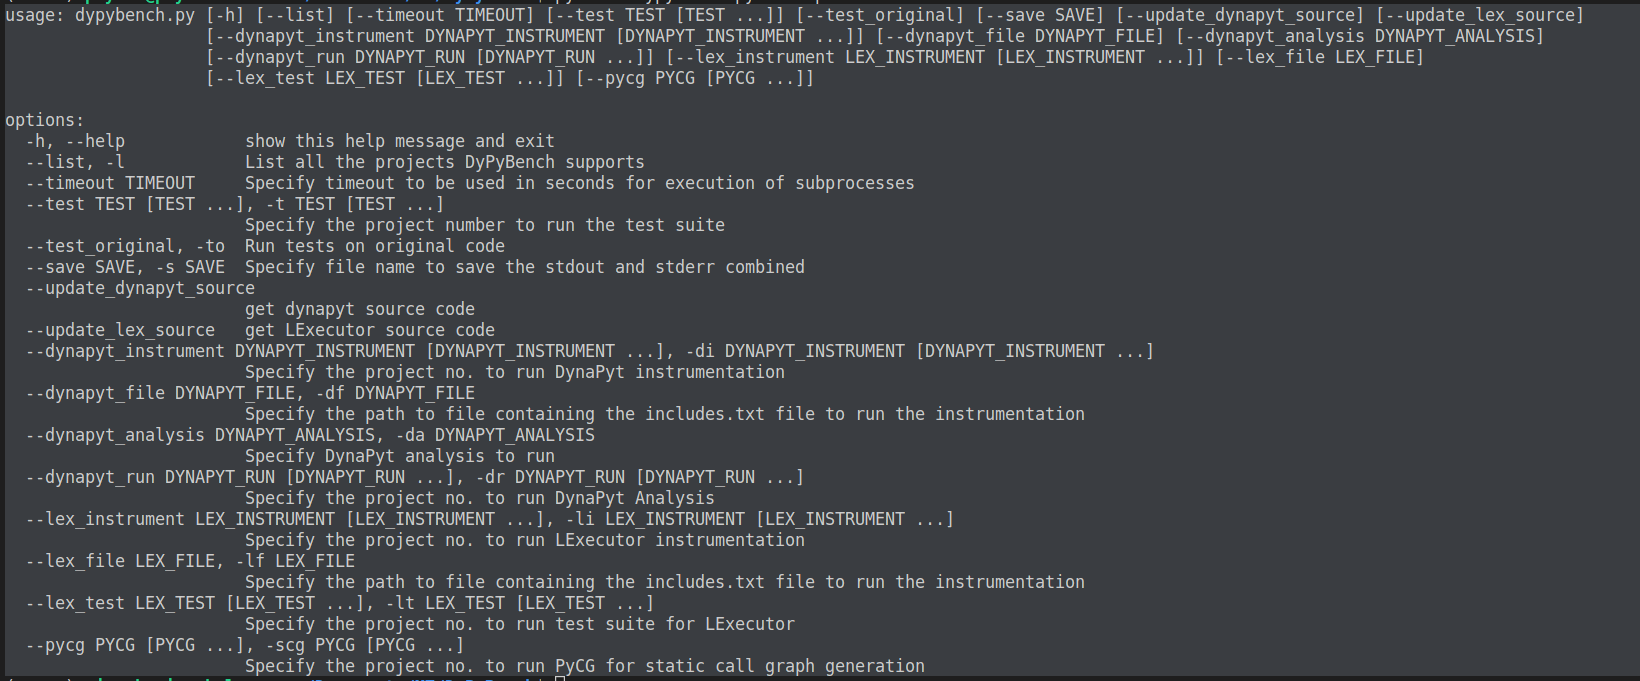
\includegraphics[width=1\linewidth]{figures/implementation/command-line-options.png}
    \caption[Command Line Options]{\label{fig:command-line-options}Command Line Options}
\end{figure}

Internally, the options except list, timeout, test\_original and save trigger the execution of a specific bash script with some arguments using the subprocess module in Python.
The list option uses the github-url.txt file to list all the projects in the benchmark.
The save option is used to save the output to a file, since we do not print the output of the executed commands on the CLI.
The timeout option kills the processes started by the python script after specified amount of seconds.
The project is specified as a number.
We can use the list command to get the mapping of project name to project number.
Multiple projects can be specified with a list of space separated numbers.
The options update\_dynapyt\_source and update\_lex\_source clone or update the source code of DynaPyt and LExecutor respectively.
In order to execute test suite, the option test is provided.
The test\_original option can be combined with test to run the test suite without creating a copy of the project to work with.
The command dynapyt\_instrument, dynapyt\_file and dynapyt\_analysis are combined to perform the task of DynaPyt instrumentation.
The first option specifies the projects, the second specifies the file to use for instrumentation and the third specifies the analysis for which the instrumentation needs to be done.
In order to perform the dynamic analysis, DynaPyt to execute these instrumented files with the options dynapyt\_run and dynapyt\_analysis combined.
The first option above specifies the projects, whereas the second specified the name of the analysis to be performed.
PyCG is generates the call graphs using the project source and the entry points.
We provide the option of pycg that accepts the project number, we then use the project root as the project source and the test files as the entry point to generate call graphs using PyCG.
LExecutor also performs its own instrumentation on the files specified.
We provide the options of lex\_instrument and lex\_file for this task.
The first specifies the projects, whereas the second specifies the file which list all the files to instrument.
To generate the trace files, LExecutor executes the test suite of the instrumented project using the option lex\_test.

\section{Integrating LExecutor and Analysis Frameworks}
For LExecutor and the analysis frameworks to work efficiently, we need to test suite that does not contain test failures.
However, the cloned projects contain some failed test cases.
In this work, we skip these failed test cases of the projects using the pytest marker.
First, we find the test cases which are failing by executing the test suite with the generic interface.
We then create a copy of the files which contain these test cases and add the pytest markers as shown in the Listing \ref{code:pytest_marker}.
The marker shown on line 1 skips the entire file from execution, whereas line 3 shows the marker that skips only the test function.
Finally, we use a python script to replace the files having failed tests cases with the files we just created.
This step of adding a skip marker and replacing the files is done during the installation process to avoid any repetition and provide ready to use projects.
\begin{lstlisting}[caption=Skip Test Case using Pytest Marker,label=code:pytest_marker,language=Python]
pytestmark = pytest.mark.skip("skip for dypybench")

@pytest.mark.skip("skip for dypybench")
\end{lstlisting}

\subsection{LExecutor}
In this work, we clone the source code of LExecutor from its repository and create a python virtual environment using the update\_lex\_source option from the access interface.
This virtual environment has LExecutor and all its dependencies installed.
LExecutor works in two steps to generate traces files, first it instruments the source code of the project and then generates trace files by executing the project.
The instrumentation is not necessarily done on all the source files, but rather the files that run during execution.
In this work, we provide the files to be instrumented in the form of a list in text file.
The text file contains a list of two space separated values, the first specifies the name of the project and the second specifies the path of the file to be instrumented.
In this work, we provide a python utility script to generate this text file, by parsing all the projects and filtering out the source files.
Certain files are excluded from this text file to avoid issues with running test suite.
The Listing \ref{code:lex_instrument.txt} shows sample entries from the above mentioned text file.
This text file is specified in the lex\_file option from the access interface.
\begin{lstlisting}[caption=lex\_instrument\_all.txt,label=code:lex_instrument.txt,language=Bash]
grab ./temp/project1/tests/test_grab_pickle.py
grab ./temp/project1/tests/test_spider_queue.py
grab ./temp/project1/tests/test_ext_rex.py
grab ./temp/project1/tests/test_grab_cookies.py
errbot ./temp/project18/errbot/core_plugins/chatRoom.py
errbot ./temp/project18/errbot/core_plugins/backup.py
errbot ./temp/project18/errbot/core_plugins/acls.py
\end{lstlisting}

The option lex\_instrument triggers a bash script to instrument the files specified in the text file.
The bash script executes the command shown in Listing \ref{code:lex_instrument} to instrument the files.
The parameter \$\{@:4\} is replaced by the space separated file paths. 
\begin{lstlisting}[caption=LExecutor Instrumentation,label=code:lex_instrument,language=Bash]
python -m lexecutor.Instrument --files ${@:4} --iids /DyPyBench/iids.json --validate
\end{lstlisting}

In order to generate the trace files, the execution of the test suite is done using another bash file.
This bash file is triggered by the option lex\_test, which simply runs the test suite using command shown in Listing \ref{code:lex_test}.
The parameter \$3 is replaced by the test suite directory specified in github-url.txt.
\begin{lstlisting}[caption=LExecutor Test Suite Execution,label=code:lex_test,language=Bash]
pytest $3
\end{lstlisting}

The instrumentation also generates a iids.json file which is used by the LExecutor to convert the traces files into training data for the neural model.
In this work, provide some utility functions related to LExecutor.
These utility functions are useful for different reasons such as gathering trace files, inspecting the output and training logs of LExecutor.

\section{PyCG}
The option pycg from the access interface triggers the execution of the bash script which first installs the pycg package to the project virtual environment and then triggers the PyCG commands as shown in the Listing \ref{code:pycg}.
Only one of the two commands is executed based on the if condition shown on line 1, which checks if the test suite is a directory or a file.
The command on line 6 specifies all the .py files in the test suite directory as the entry point for the call graphs.
\begin{lstlisting}[caption=PyCG Execution,label=code:pycg,language=Bash]
if [[ $4 == "file" ]]
then
    pycg --package ./project$2 project$2/$3 -o pycg_$2.json
elif [[ $4 == "folder" ]]
then
    pycg --package ./project$2 $(find project$2/$3 -type f -name "*.py") -o pycg_$2.json
fi
\end{lstlisting}

As we can see from the Listing \ref{code:pycg}, the output file is generated for each project in the project folder.
To collect these JSON output files, we provide a utility function to collect them for further analysis.  

\section{DynaPyt}
In this work, we clone the source code of DynaPyt from its repository using the update\_dynapyt\_source option from the access interface.
DynaPyt, first needs to instrument the source files and then execute these instrumented files to provide the results of analysis.
DynaPyt provides the options to instrument a directory or files.
It is also possible to specify which files or directory we need to instrument.
We provide a text file which contains the list of directories and files which we want to instrument.
This text file, has 3 space separated values on each line.
The first value is the project name, whereas the second value is the flag indicating file or directory.
The possible values for this flag are f for file and d for directory.
Lastly, the third value in the space separated entry is the directory or the file path, relative to the root of the project to be instrumented.
Listing \ref{code:dynapyt_instrument.txt} shows some sample entries from this file.

\begin{lstlisting}[caption=dynapyt\_instrument\_all.txt,label=code:dynapyt_instrument.txt,language=Bash]
flask-api d ./flask_api
schedule d ./schedule
schedule f ./test_schedule.py
Pillow d ./src
Pillow d ./Tests
supervisor d ./supervisor
streamparse d ./streamparse
\end{lstlisting}

In this work, we provide two such text files for instrumentation, one which includes all the source files and the test files and the other which excludes test files.
To instrument the code, the bash script first copies the DynaPyt source code that was cloned to the specific project directory.
Then, DynaPyt is installed with its dependencies into the virtual environment of the specific project.
Finally, the bash script runs the command to instrument the files or folder based on the flag provided by the above mentioned text file.
The instrumentation is based on the hooks provided by DynaPyt for the particular analysis.
Therefore, we need to provide the name of the analysis to be performed.
We provide this with the option dynapyt\_analysis to the access interface.
The two instrumentation commands are shown in the Listing \ref{code:dynapyt_instrument}. 
\begin{lstlisting}[caption=DynaPyt Instrumentation,label=code:dynapyt_instrument,language=Bash]
if [[ $5 == "d" ]]
then
    #run instrumentation on the given directory
    python -m dynapyt.run_instrumentation --directory $3 --analysis $4
elif [[ $5 == "f" ]]
then
    #run instrumentation on the given file
    python -m dynapyt.instrument.instrument --files $3 --analysis $4
fi
\end{lstlisting}

The execution of test suite to perform the dynamic analysis is done using another bash script.
We first create an entry file to run all the tests with pytest with the parameter import-mode set to importlib.
We then trigger the execution of tests with run\_analysis module provided by dynapyt, specifiying the above entry file and the name of the analysis.
Listing \ref{code:dynapyt_test} shows the creation of the entry file on line 1 and execution with run\_analysis on line 3.
\begin{lstlisting}[caption=DynaPyt Test Suite Execution,label=code:dynapyt_test,language=Bash]
printf "import pytest\n\npytest.main(['--import-mode=importlib', '$ROOT_DIR/temp/project$2/$4'])\n" > run_all_tests.py

python -m dynapyt.run_analysis --entry ./run_all_tests.py --analysis $3
\end{lstlisting}

In this work, we developed a new analysis named CallGraph to generate call graphs during run-time.
This code for this analysis is shown in Listing \ref{code:CallGraphAnalysis}.
We use the function pre\_call hook provided by DynaPyt and create the call graph in the form of dictionary.
A keys in this dictionary is the fully qualified names of the caller method and the value for this key is a list of fully qualified names of called methods.
At the end of the execution, we output the dictionary to a JSON file.
A utility function is provided in this work to collect all the JSON files from the projects that were dynamically analyzed.